Deciding how a simulation is structured from an interactions standpoint is a
delicate balance of known necessity and perceived future needs. There are basic
decisions to make: do you want a system with discrete material transfers or
continuous material flows? Discrete transfers more closely match reality and may
provide insights in that regard, however they require more of their modeling
apparatus due to messaging needs and other structures. More complex decisions
include how one wants to determine connections between facilities. Does one
assign supplier-consumer pairs to facilities? Does one allow them to change?
Should the facility make such a decision? Should that decision be affected by
any other entities? Guerin's comment in \S\ref{sec:intro-benchmarks} stems from
this ``freedom''. These simulation-engine decisions comprise the art-related
portion of fuel cycle simulation, but developers have a goal of making these
decisions in as informed a way as possible using domain-level knowledge with
respect to our known and perceived requirements. In general, this work tries to
minimize the sheer number of choices we make in this regard, instead relying on
well known and well documented practices of computer scientists and systems
engineers.

The \Cyclus team is also interested in fostering a user and developer ecosystem.
Accordingly, such concerns also drive the simulation architecture design. The
agent-based nature of \Cyclus provides an opportunity to reduce barriers to
entry into the ecosystem. Given a few basic tenets of agent interaction, other
developers should be able to create a new agent to ``plug in'' to the
simulation. Intuitively, a minimal set of behaviors must be defined to
sufficiently inform the simulation infrastructure to run the simulation. This
freedom allows the simulation program introduce agents at run time, effectively
separating the simulation engine's functionality from the agents in the
simulation.

Such a framework provides many benefits. First, there is a clear separation of
concerns. The \Cyclus core is concerned with modeling system dynamics whereas
individual agents are concerned with domain-specific issues. Accordingly,
developers can focus their attention appropriately, focusing either on the core
code base or on agent development. Separating agent development from core
development also allows \Cyclus to remain a viable open-source candidate to
model nuclear fuel cycle dynamics. Because domain-level information is
incorporated into agent libraries which are dynamically loaded at runtime, a
closed-source developer can focus their efforts entirely on developing agent
libraries. Furthermore, developers could participate both privately and
publicly, e.g., adding general capability to the \Cyclus core that is needed for
some functionality without specifying the internals. Such a community paradigm
is shown in Figure \ref{fig:community}.

\begin{figure}[htbp!]
  \begin{center}
    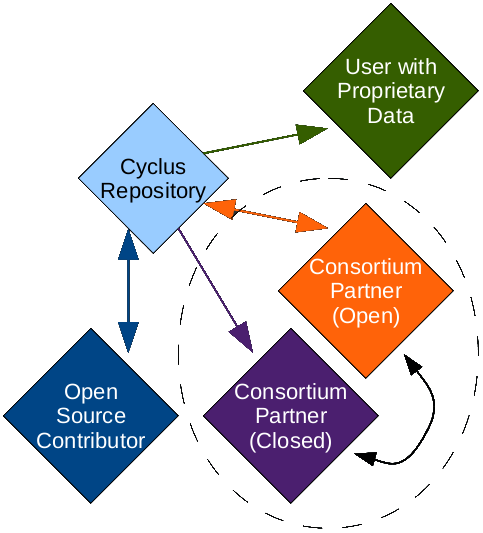
\includegraphics[height=8cm]{./chapters/research/community.png}
  \end{center}
  \caption{The Cyclus Participation Paradigm} 
  \label{fig:community}
\end{figure}

In order to develop and maintain the core code separate from the agent modules,
well-defined interactions must be provided between agents and the \Cyclus
core. The remaining part of the section provides a proposal for such
interactions that allow for a variety facility deployment and supply-demand
matching algorithms to be employed. A description of the market resolution
interface is provided, and basic agent simulation interaction, such as entering
and leaving the simulation is also described.

\subsection{Supply-Demand Framework}

The resolution of supply and demand at any given time step is the result of the
mathematical program techniques described in \S\ref{sec:gfctp}. The method of
providing information to solution engine, however, is a simulation-interaction
mechanism that must be developed. Supply-demand determination at any given time
step occurs in nominally three steps, or \textit{phases}, and the terminology of
this ``phase space'' is taken from previous supply chain agent-based modeling
work \cite{julka_agent-based_2002}. Importantly, this information-gathering step
is agnostic as to the actual matching algorithm used, it is concerned only with
querying the current status of supply and demand in the simulation.

The first phase allows consumers of commodities to denote both the quantity of a
commodity they need to consume as well as the target isotopics, or quality, by
\textit{posting} their demand to the market exchange. This posting informs
producers of commodities what is needed by consumers, and is termed the
\textit{Request for Bids} (RFB) phase. Consumers are allowed to over-post, i.e.,
request more quantity than they can actually consume, as long as a corresponding
capacity constraint accompanies this posting. Further, consumers are allowed to
post demand for multiple commodities that may serve to meet the same combine
capacity. For example, consider an LWR that can be filled with MOX or UOX. It
can post a demand for both, but must define a preference over the set of
possible commodities it can consume. Another example is that of an advanced fuel
fabrication facility, i.e., one that fabricates fuel partially from separated
material that has already passed through a reactor. Such a facility can choose
to fill the remaining space in a certain assembly with various types of fertile
material, including depleted uranium from enrichment or reprocessed uranium from
separations. Accordingly, it could demand both commodities as long as it
provides a corresponding constraint with respect to total consumption. At the
completion of the RFB phase, the market exchange will have a set of consumption
portfolios, $P$, where each portfolio consists of a set requests, $R$, a
cardinal preference over the requests, $\alpha_R$, and possibly a set of
constraints over the requests, $C_R$. Each request consists of a quantity,
$q_r$, and a target isotopic vector, $I_r$.

The second phase allows suppliers to \textit{respond} to the set of consumption
portfolios, and is termed the \textit{Bidding} (B) phase (analgous to Julka's
Reply to Request for Quote phase \cite{julka_agent-based_2002}). Each
consumption portfolio is comprised of requests for some set of
commodities. Accordingly, for each request, suppliers of that commodity denote
production capacities and an isotopic profile of the commodity they can
provide. Suppliers are allowed to offer the null set of isotopics as their
profile, effectively providing no information. A supplier may have its
production constrained by more than one parameter. For example, a processing
facility may have both a throughput constraint (i.e., it can only process
material at a certain rate) and an inventory constraint (i.e., it can only hold
some total material). Further, the facility could have a constraint on the
quality of material to be processed, e.g., it may be able to handle a maximum
radiotoxicity for any given time step which is a function of both the quantity
of material in processes and the isotopic content of that material. The
formulation provided in \S\ref{sec:gfctp} allows for multiple of such
constraints as long as they are linear functions of the demanded commodity
quantity. At the completion of the Bidding phase the possible connections
between supplier and producer facilities, i.e., the arcs in the graph of the
transportation problem, have been established with specific capacity constraints
defined both by the quantity and quality of commodities that will traverse the
arcs.

The final phase of the information gathering procedure allows consumer
facilities to adjust their set of preferences and for managers of consumer
facilities to affect the consumer's set of preferences, as described in the
remaining sections. Accordingly, the last phase is termed the \textit{Preference
 Adjustment} (PA) phase. Preference adjustments can occur in response to the
set of responses provided by producer facilities. Consider the example of a
reactor facility that requests two fuel types, MOX and UOX. It may get two
responses to its request for MOX, each with different isotopic profiles of the
MOX that can be provided. It can then assign preference values over this set of
potential MOX providers. Another prime example is in the case of repositories. A
repository may have a defined preference of material to accept based upon its
heat load or radiotoxicity, both of which are functions of the quality, or
isotopics, of a material. In certain simulators, limits on fuel entering a
repository are imposed based upon the amount of time that has elapsed since the
fuel has exited a reactor, which can be assessed during this phase. The time
constraint is, in actuality, a constraint on heat load or radiotoxicity (one
must let enough of the fission products decay). A repository could analyze
possible input fuel isotopics and set the arc preference of any that violate a
given rule to 0, effectively eliminating that arc.

\subsection{Facilities}

Facilities in \Cyclus are abstracted to either consumers or suppliers of
commodities, and some may be both. Supplier agents are provided agency by being
able to communicate to the market-resolution mechanism a variety of production
capacity constraints in second phase of the information gathering
methodology. Consumer agents are provided agency by being able to assign
preferences among possible suppliers based on the supplier's quality of
product. Because this agency is encapsulated for each agent, it is possible to
define strategies that can be attached or detached to the agents at
run-time. Such strategies are an example of the Strategy design pattern
\cite{vlissides_design_1995}.

\subsection{Institutions}

Institutions in \Cyclus manage a set of facilities. Facility management is
nominally split into two main categories: the commissioning and decommissioning
of facilities and supply-demand association. The goal of including a notion of
institutions is to allow an increased level of detail when investigating
regional-specific scenarios. For example, there exist multi-national
enterprises, such as AREVA, that operate fuel cycle facilities in a variety of
countries, or regions. Furthermore, there are international governmental
organizations, such as the IAEA, have proposed managing large fuel cycle
facilities that service many countries in a given global region. A fuel bank is
an example of such a facility. Accordingly, institutions in \Cyclus are able to
augment the preferences of supplier-consumer pairs that have been established in
order to simulate a mutual preference to trade material within an
institution. Of course, situations arise in real life where an institution has
the capability to service its own facilities, but choose to use an outside
provider because of either cost or time constraints. Such a situation is allowed
in this framework as well. It is not clear how such a relationship should be
instantiated and to what degree institutions should be allowed to affect their
managed facilities' preferences. This issue lies squarely in the realm of
simulation design decisions, part of the \textit{art} of
simulation. Accordingly, through the course of research, the possible design
space will be analyzed in order to determine best practices for this type of
design.

\subsection{Regions}

Regions in \Cyclus provide the forcing function for simulations by requiring
that certain parameters be met, e.g., power capacity, fuel cycle service
capacity, etc. For example, in the case of nuclear power capacity, a region
knows that it needs additional reactors to be built, but leaves the building of
those reactors to the institutions that operate in the region. The current
Region model in the \Cyclus code base takes the cost and nameplate capacity for
each facility in a set of acceptable facilities and a demand gap, and solves a
minimum-cost capacity production problem to determine the number and type of
facilities to request. It is important to note here that this abstraction allows
for different deployment algorithms to be tested and exchanged in the \Cyclus
framework without necessitating changes to the simulation engine, as is the case
with other simulators described in \S\ref{sec:simulators} and is consistent with
the types of simulation design decisions described in
\S\ref{sec:simulators-overview}. 

Regions are further provided agency by their ability to affect preferences
between supplier-consumer facility pairs in the third phase of the market
information gathering algorithm. The ability to perturb arc preferences between
a given supplier and a given consumer allows fuel cycle simulation developers to
model relatively complex interactions at a regional level, such as tariffs and
sanctions. Constraints to cross-border trading can also be applied to the
formulation described in \S\ref{sec:gfctp}. For example, a region could place
constraints on the total amount of a given commodity type that is able to flow
into it or out of it into a different region. Such constraints could applied not
only to bulk quantities of a commodity, but also to the quality of each
commodity. Such a mechanism could be used to model interdiction of
highly-enriched uranium transport, for example.
